\section{Actualizar la lista de partidas}

\begin{figure}[ht]
\centering
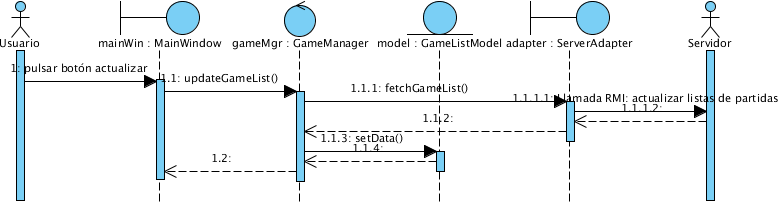
\includegraphics[scale=0.6]{img/ch03devel-listgames.png}
\caption{Diagrama de secuencia de Actualizar la lista de partidas''}
\end{figure}

Estando en la ventana principal, el usuario puede realizar una serie de
acciones. Una de ellas puede ser actualizar la lista de partidas mostrada. Ante
esta acción, el gestor de partidas solicitará una nueva lista al servidor a
través del \texttt{ServerAdapter}.

La lista recibida desde el servidor debe ser filtrada y organizada en dos
sublistas: una con partidas abiertas para unirse, y otra con partidas en las
que esté participando el usuario y estén activas en este momento.

Una vez seleccionadas las partidas, éstas son asignadas a dos objetos de tipo
\texttt{GameListModel}. Puesto que las vistas, dos \texttt{JTable}, han sido
configuradas como observadores de estos modelos, su actualización es llevada a
cabo por el \textit{framework} automáticamente.
